\newcommand{\basedir}{fablab-document}
\documentclass{\basedir/fablab-document}

\usepackage{minitoc} % Inhaltsübersicht je Section
% \usepackage{fancybox} %ovale Boxen für Knöpfe - nicht mehr benötigt
\usepackage{amssymb} % Symbole für Knöpfe
% \usepackage{subfigure,caption}
\usepackage{eurosym}
\usepackage{tabularx} % Tabellen mit bestimmtem Breitenverhältnis der Spalten
\usepackage{wrapfig} % Textumlauf um Bilder
\usepackage{todonotes}
\usepackage{framed}
\usepackage{xargs}
\usepackage{framed}
\renewenvironmentx{leftbar}[3][2=0.5pt, 3=5pt]{\def\FrameCommand{\vrule width #2 \hspace{#3}}\MakeFramed {\advance\hsize-\width \FrameRestore}{\tiny#1\\}} {\endMakeFramed}

\renewcommand{\texteuro}{\euro}

\renewcommand{\todo}[1]{\textbf{\color{red}{TODO: #1}}}

\linespread{1.2}

\date{April 2020}
\author{FAU FabLab}
\title{Einweisung Shaper Origin}

\begin{document}
 % Hinweise an Package minitoc, doch bitte irgendwas zu generieren - wird für späteres \secttoc benötigt
\dosecttoc
\faketableofcontents
\mtcsettitle{secttoc}{Arbeitsschritte}
\mtcsettitlefont{secttoc}{\large \sffamily \bfseries}
\mtcsetfont{secttoc}{subsection}{\sffamily}
% \mtcset
% hier geht das eigentliche Dokument los

%\color{red}
%\hrule
%\begin{center}
%\large{Achtung! Einweisung ist noch in Arbeit!}
%\vspace{0.1cm}
%\end{center}
%\hrule
%\color{black}



\section{Technische Daten}
\begin{description}
    \item[Hersteller] Shapertools
    \item[Produktname] Origin
    %\item[Leistung] $-----\,\mathrm{Watt}$
    \item[Drezahlbereich] 10.000 (Stufe 1) - 26.000 (Stufe 6)$\,\mathrm{min}^{-1}$
    %\item[Fräserdurchmesser] max. $-----\,\mathrm{mm}$
    \item[Fräserschaftdurchmesser] Festtool Spannzangen: Standard: 8mm
\end{description}


\section[Allgemeine Sicherheitshinweise]{Allgemeine Sicherheitshinweise}
\begin{itemize}
    \item Werkstück immer gut festspannen oder auf festgespannter Unterlage
        mit doppelseitigem Tape festkleben, nie in der Hand oder von Dritten
        halten lassen oder auf dem Tisch festkleben
    \item Maschine beim Fräßen stets an beiden Griffen halten und führen
    \item Die Maschine stellt sicher, dass immer im Gegenlauf gefräst wird
    \item Der Origin taucht erst ein, wenn die Spindel läuft
    \item Vor Werkzeugwechsel Spindel vom Origin trennen -- Stecker ziehen
    \item Werkzeug fest einspannen -- dazu Schlüssel aus der Maschinenkiste oder
        19mm Maulschlüssel verwenden
    \item Keine defekten, rissigen, verbogenen oder stumpfen Werkzeuge verwenden
    \item Unbedingt mit aktivem Staubsauger fräsen
    \item Netzkabel aus dem Eingriffsbereich des Fräsers halten
    \item Nach dem Fräsen Maschine reinigen und aussaugen. Zum abblasen mit Druckluft,
        Maschine aus dem Fenster halten
    \item Im Arbeitsbereich dürfen sich keine Unbeteiligten befinden
    \item Maximale Frästiefe je Fräsgang bei Holz: 1 x Fräser-\o\ -- Brandgefahr!
    \item Ausreichend Vorschub bzw.\ nicht zu hohe Drehzahl verwenden, da sonst
        der Fräser ausglüht.
\end{itemize}


\section{Persönliche Schutzausrüstung}
\begin{itemize}
    \item Gehörschutz -- hängt an der Fräse, links neben der Werkbank
    \item Schutzbrille -- hängen hinter der Werkbank und hinter dem
        Chemiearbeitsbereich an der Wand
    \item Staubmaske bei stauberzeugenden Arbeiten (besonders
        Hartholz) -- liegen in der Schutzausrüstungsschublade W9
    \item Fingerschutz um den unteren Teil der Spindel
    \item Bewusstes Wahrnehmen des nächsten Not-Aus Knopfes
    \item Lange Haare müssen sicher zurückgebunden sein
    \item Pulloverkordeln müssen in den Pullover gesteckt werden
    \item Geschlossene Schuhe tragen
\end{itemize}

%\begin{figure}[h!]
%    \centering
%    \includegraphics[width=0.8\textwidth]{bilder/shaper_front}
%    \caption{Shaper Ansicht vorne}
%    \label{fig:sketch}
%\end{figure}

%\begin{figure}[h!]
%    \centering
%    \includegraphics[width=0.8\textwidth]{bilder/shaper_side}
%    \caption{Shaper Ansicht Seite}
%    \label{fig:sketch2}
%\end{figure}

\section{Vor der ersten Benutzung}
Shaper stellt die dem Origin beiliegende Kurzstartanleitung zur Verfügung.
Diese ist durchzulesen! Darin wird auch das Kleben der Tapestreifen erklärt.
Ebenfalls sollten unter folgendem Link die Videos angeschaut werden:
\url{www.shapertools.com/start} Hier werden die Grundlagen erklärt.
Ergänzend sollten bereits eingewiesene und erfahrene Personen bei der ersten
Nutzung anwesend sein und diese nochmals erklären und überprüfen.
Einen Überblick dieser findest du am Ende dieser Einweisung.

\section{Bestimmungsgemäße Verwendung}
Der Shaper Origin ist zur Bearbeitung von Kanten, zum Versäubern und auch
zur kreativen Gestaltung (z.\,B.\ Einfräsen von Schrift oder Löchern in
Plattenmaterial). Es ist wichtig, die folgenden Anweisungen genau zu
beachten, damit der Origin nicht zu Gesundheitsschäden führt oder
beschädigt wird.\\
Es dürfen mit der Maschine Holz, Kunststoff und (Aluminium) bearbeitet
werden, dabei immer auf die richtige Fräserauswahl, Spindeleinstellung,
Tiefeneinstellung und Vorschub achten. Unter
\url{https://support.shapertools.com/hc/en-us/categories/115000254454-Using-Origin}
gibt es Werte zur Orientierung. Bei der Verwendung der Maschine
muss der Festool-Staubsauger verwendet werden, da sonst sehr viel
Staub und Dreck entsteht. Dabei ist zu beachten, dass der Origin entweder
an einer Steckdose des Festool-Saugers angeschlossen wird und der Sauger
selbst auf \enquote{AUTO} sowie voller Saugleistung steht oder der
Staubsauger durchgängig an ist. Bei Holz kann sich der Einlass der Absaugung
an dem Origin durch Holzsplitter zusetzen. Bei geringem Absaugeffekt ist
die Arbeit zu unterbrechen und die Problemstelle zu finden.\\
\textbf{WICHTIG: Der Shaper darf ausschließlich von eingewiesenen Personen verwendet werden.}

\subsection{Arbeiten während Openlabs}
Ob die Maschine während openlabs genutzt werden kann, entscheiden die anwesenden
Betreuer. Dies geht nur, wenn wenige Personen anwesend sind, alle
entsprechenden Gehörschutz tragen und es keine Personen stört.
Während der Vorlesungszeit / Klausurenzeit ist darauf zu achten,
das die Labtüren geschlossen sind.

\section{Nach der Benutzung}
\begin{itemize}
\item Die Maschine ist mit Druckluft und Staubsauger zu reinigen
\item Nach dem fräsen von Holz bei Bedarf den Fräser mit Harzentferner reinigen
\end{itemize}

\section{Einstellungen}
\subsection{Funktionen der Maschine}
\begin{itemize}
    \item Konstante Drehzahl: Die Motordrehzahl wird elektronisch konstant gehalten.
        Dadurch wird auch bei Belastung eine gleichbleibende Schnittgeschwindigkeit erreicht.
    \item Drehzahlregelung: Die Drehzahl lässt sich mit dem Stellrad an der Spindel
        stufenlos einstellen. Dadurch können die Schnittgeschwindigkeit der jeweiligen
        Oberfläche optimal angepasst werden
    \item Temperatursicherung: Bei zu hoher Motortemperatur werden Stromzufuhr
        und Drehzahl reduziert. Die Maschine läuft nur noch mit verringerter
        Leistung, um eine rasche Abkühlung durch die Motorlüftung zu ermöglichen.
    \item Strombegrenzung: Die Strombegrenzung verhindert bei extremer Überlastung
        eine zu hohe Stromaufnahme. Dies kann zu einer Verringerung der Motordrehzahl
        führen. Nach Entlastung läuft der Motor sofort wieder an.
    \item Die Software des Origin verhindert das Verlassen des Fräspfades.
    \item Die Software gibt die Fräsrichtung vor, es gilt den Anweisungen der Software folge zu leisten.
    \item Die Maschine führt den Fräser selbstständig auf der Linie. Um ein
        gutes Ergebnis zu erzielen kann der Auto-Modus genutzt werden, in dem ein
        gleichbleibender Vorschub gewährleistet wird.
\end{itemize}

\subsubsection{Fräser wechseln}
siehe beiliegende Schnellstart Anleitung.

\subsection{Frästiefe einstellen}
Der Shaper verfügt über das Menü Fräserwechsel, in dem nach einem Durchmesser-
oder Typwechsel die automatische Neukalibrierung abgefragt wird. Wichtig dabei
ist, während des Vorgangs den Origin am besten nicht anzufassen.

\subsection{Drehzahl wählen}
Über das Stellrad an der Spindel wird die Drehzahl gewählt, diese hängt vom
Material des Werkstücks und dem Fräser ab. Siehe Abbildung~\ref{fig:drehzahl}
für Hersteller Empfehlungen für die Oberfräse von Festtool. Diese dürften
-- nicht validiert! -- auch für den Origin passend sein.
\begin{figure}[h!]
    \centering
    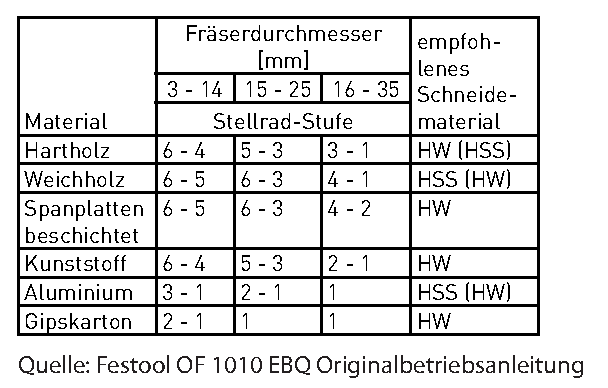
\includegraphics{img/drehzahltabelle.pdf}
    \caption{Drehzahltabelle}
    \label{fig:drehzahl}
\end{figure}

\section{Arbeiten mit der Maschine}
Beim Arbeiten mit der Maschine ist das Werkstück stets festzuspannen
und gegen Verrutschen zu sichern. Die Maschine muss mit beiden Händen gehalten
werden. Bei Arbeiten, die gefährliche Stäube erzeugen, ist der Staubsauger
auf maximale Leistung einzustellen. Hierzu zählt auch Hartholz (vor allem
Buche und Eiche sind nachweislich krebserregend recht unabhängig von der Expositionsdauer)!

Tipps zum Festspannen:
\begin{itemize}
    \item zu fräsende Objekte gut auf einer festgespannten Grundplatte mit
        doppelseitigem Tape festkleben. Wichtig: Alle Teile die ausgeschnitten werden
        sollen, müssen ebenfalls mit Tape verklebt sein, da sie andernfalls am
        Ende verrutschen und dadurch eine Gefahr darstellen
    \item Fräsertiefe beachten.
    \item Shapertape auf einer der vorgefertigten Platten nutzen oder eigene
        Platte erstellen. Diese dann oberflächenschlüssig vor das Werkstück
        befestigen. Diese müssen gegen verrutschen zum Werkstück gesichert
        werden, da andernfalls das Werkstück kaputt geht!
\end{itemize}

Tipps für gute Ergebnisse bei Holz:
\begin{itemize}
    \item Rechtwinklig zur Faserstruktur Vorschub leisten. Dies verhindert
        das Splittern des Holzes entlang der Maserung.
    \item Für den Außengebrauch steht ein Festtool Arbeitstisch zum
        ausklappen bereit. Wende dich dafür an einen Betreuer.
    \item Richtige Spindeldrehzahl wählen.
    \item Wenn möglich Origin in der gleichen Richtung beim Fräsen
        halten, in der gescannt wurde.
\end{itemize}

Weiteres ist in der Kurzanleitung.

\subsection{Aluminium, Kupfer, ... (nicht eisenhaltige Metalle)}
Das Bearbeiten von nicht eisenhaltigen Metallen ist nur fortgeschrittenen
Benutzern erlaubt. Hierbei muss beim ersten mal fräsen ein Betreuer anwesend
sein, der ebenfalls mit nicht eisenhaltigen Metallen am Origin bereits gearbeitet hat.

%\newpage
\section{Quellen und Rechte}
\label{quellen}
Alle Rechte an Grafiken, Tabellen und Textabschnitte, welche aus der Shaper
Originalbetriebsanleitung übernommen wurden, liegen bei Shapertools. Die
\enquote{Originalbetriebsanleitung} liegt der Maschine bei und ist online auf
\url{https://assets.shapertools.com/manual/Shaper_Origin_Product_Manual.pdf}
zu finden. Shapertools hat dieses Dokument weder gelesen, noch auf Vollständigkeit
oder Richtigkeit geprüft und übernimmt keine Haftung.
Gleiches gilt für die Tabelle aus der Festtool Oberfräseneinweisung.
%\begin{itemize}
%\item Festool \glqq Originalbetriebsanleitung\grqq TS 55 REBQ unter
%\url{http://www.etracker.de/lnkcnt.php?et=6hsNGE&url=https\%3a\%2f\%2fassets.festool.com\%2fmedia\%2f706758_002_ts55rebq.zip&lnkname=Bedienungsanleitung+TS+55}
%\end{itemize}

Dieses Dokument stammt aus fau-fablab/shaper-origin-einweisung@\Revision{}.

\todo{Klären, ob und wo CC-Lizenz gesetzt werden kann, dann ccLicense-Block einbinden.}
%\ccLicense{shaper-origin-einweisung}{Einweisung Shaper Origin}

\end{document}
